\documentclass{article}
\usepackage{amsmath}
\usepackage{mathtools}
\usepackage{gensymb}
\usepackage[a4paper,inner=1.5cm,outer=1.5cm,top=2cm,bottom=0.5cm]{geometry} 
\usepackage{xcolor}                    
\usepackage{tikz}                           
\usepackage{multicol}
\usepackage{pgfplots}
\usetikzlibrary{calc}
\usetikzlibrary{intersections}
\usetikzlibrary{intersections,calc,angles,quotes}
\usetikzlibrary{shapes,arrows,positioning,decorations.pathreplacing,calc}
\usetikzlibrary{calc,angles,positioning,intersections,quotes,decorations.markings}
\usepackage{tkz-euclide}
\usetikzlibrary{backgrounds}
\usetikzlibrary{calc,through}
\usetikzlibrary{angles}
\usetikzlibrary{fadings}
\usetikzlibrary{shapes.geometric}
\usetikzlibrary{shapes.symbols}
\usepackage{draftwatermark}
\usepackage{mathptmx}

\SetWatermarkText{\textcolor{black!30}{Mathema Shukur}}
\SetWatermarkFontSize{2 cm}
\usepackage[utf8]{inputenc}
\usepackage{fontspec}

\setmainfont{[Kalpurush.ttf]}
\newfontface{\en}{[Arial.ttf]} %%this is optional, if you want to use a secondary font. Any english font is supported
\newlength\Radius
\setlength\Radius{4cm}
\begin{document} 
	\Large
	\textcolor{red}{Welcome To} 
	\\
	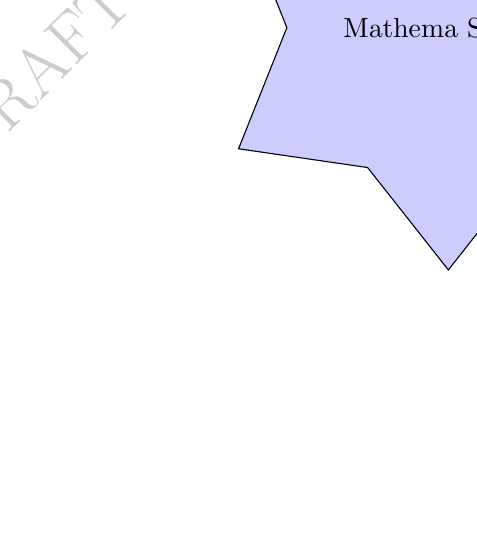
\begin{tikzpicture}
		\tikz \node [fill=blue!20,star,star points=6,draw] {Mathema Shukur };
	\end{tikzpicture}
	\\
	যাদের জন্যে প্রযোজ্যঃ  	\textcolor{magenta}{একাদশ ও দ্বাদশ শ্রেণীর শিক্ষার্থী} \\
	বিষয়ঃ \textcolor{magenta}{উচ্চতর গণিত ১ম পত্র} \\
	অধ্যায়ঃ \textcolor{magenta}{৩-সরলরেখা}\\ 
	Subtopicঃ  \textcolor{magenta}{  দুইটি সরলরেখা পরস্পর লম্ব হওয়ার শর্ত   }\\
	\\
	দুইটি সরলরেখা পরস্পর লম্ব হবে যদি রেখাদ্বয়ের অন্তর্গত কোণ  সমকোণ $(90\degree)$ হয় \\
	\\ 
	ঢাল খন্ডন আকার সমীকরণ\\
	$y=m_1x+c_1$ এবং $y=m_2x+c_2$ সরলরেখা দুইটি পরস্পর লম্ব হবে যদি রেখাদ্বয়ের অন্তর্গত কোণ  সমকোণ $(90\degree)$ হয় \\
	\\ 
	\begin{align*}
		\tan \theta  &= \frac{m_1-m_2}{1+m_1\,\,m_2}\\
		\\
		\tan  90  &= \frac{m_1-m_2}{1+m_1\,\,m_2}\\
		\\
	\cot	90 &= \frac{1+m_1\,\,m_2}{m_1-m_2}\\
		\\
	0 &= \frac{1+m_1\,\,m_2}{m_1-m_2}\\
		\\
	1+m_1\,\,m_2&=0\\
	\\
	m_1\,\,m_2&=-1
	\end{align*}
	\\
	দুইটি সরলরেখা পরস্পর লম্ব  হবে যদি  রেখাদ্বয়ের  ঢাল দুইটির গুণফল $-1$ হয় \\
	\\ 
	আদর্শ আকার সমীকরণের ক্ষেত্রে \\
	$a_1x+b_1y+c_1=0$  সরলরেখার ঢাল  $m_1=-\frac{a_1}{b_1}$\\
	\\
	$a_2x+b_2y+c_2=0$  সরলরেখার ঢাল  $m_2=-\frac{a_2}{b_2}$\\
	\\
	$a_1x+b_1y+c_1=0$ এবং 	$a_2x+b_2y+c_2=0$  সরলরেখা পরস্পর লম্ব  হবে যদি  রেখাদ্বয়ের  ঢাল দুইটির গুণফল $-1$ হয় \\
	\\
	\begin{align*}
	m_1\,\,m_2&=-1
		\\
	\left(	-\frac{a_1}{b_1}\right)\,\,\left(-\frac{a_2}{b_2}\right)&=-1\\
		\\
		\frac{a_1\,\,a_2}{b_1\,\,b_2}&=-1\\
		\\
		a_1\,\,a_2&=-b_1\,\,b_2\\
		\\
		a_1\,\,a_2+b_1\,\,b_2&=0
	\end{align*}
	\\
	\textcolor{blue}{	$y=m_1x+c_1$ এবং $y=m_2x+c_2$  সরলরেখা পরস্পর লম্ব  হবে যদি যদি $	m_1\times m_2=-1$ হয় (ঢাল আকার শর্ত) }\\
	\\
	\textcolor{red}{$a_1x+b_1y+c_1=0$ এবং 	$a_2x+b_2y+c_2=0$  সরলরেখা পরস্পর লম্ব  হবে যদি যদি $	a_1\,\,a_2+b_1\,\,b_2=0$ হয় (সহগ আকার শর্ত) }\\
	\\
	চট্রগ্রাম বোর্ড-২০২২\\ 
 $4x-3y-51=0$ সরলরেখার উপর লম্ব রেখার ঢাল কত? । \\ 
	\\
 $4x-3y-51=0$ সরলরেখারঢাল  $m_1=-\frac{4}{-3}=\frac{4}{3}$\\
	\\
 ধরি, $4x-3y-51=0$ সরলরেখার উপর লম্ব রেখার ঢাল   $m_2$\\
	\\
লম্ব হওয়ার ঢাল আকার শর্ত \\ 
	\\
	\begin{align*}
		m_1\times m_2&=-1\\
		\\
	\left(\frac{4}{3}\right)\,\,m_2&=-1\\
		\\
		m_2&=-\frac{3}{4}
	\end{align*}
	\\
	$4x-3y-51=0$ সরলরেখার উপর লম্ব রেখার ঢাল   $-\frac{3}{4}$ \\
	\\ 
	দিনাজপুর  বোর্ড-২০২১\\
	$2x+5y+1=0$	ও $-kx+10y-3=0$ রেখাদ্বয় পরস্পর লম্ব হলে $k$ এর  মান কত? \\
	\begin{multicols}{2}
		\begin{align*}
		2x+5y+1&=0\\
			\\
			a_1=2,\quad b_1=5,\quad c_1=1
		\end{align*}
		\\
		\begin{align*}
		-kx+10y-3&=0\\
			\\
			a_2=-k,\quad b_2=10,\quad c_2=-3
		\end{align*}
	\end{multicols}
	লম্ব হওয়ার সহগ আকার শর্ত \\
	\begin{align*}
		a_1\,\,a_2+b_1\,\,b_2& =0\\
		\\
	(2)(-k)+(5)(10)&=0\\
		\\
	-2k+50&=0\\
	\\
	-2k&=-50\\
	\\
	k&=\frac{50}{2}\\
	\\
	k&=25
	\end{align*}
	\\
	\\
	\begin{tikzpicture}[transform shape,scale=1]
		\draw [-latex,thick](-5,0) -- (5,0) node[right] {$x$} coordinate(x axis);
		\draw [-latex,thick](0,-4) -- (0,6) node[above] {$y$} coordinate(y axis);
		\fill[black] (0,0) circle (1 mm);
		\node at (0.3,-0.3) {$\textcolor{purple}{O}$};	
		\node at (3,3) {$\textcolor{blue}{-25x+10y-3=0}$};	
		\node at (6,-2.5) {$\textcolor{green}{2x+5y+1=0}$};	
			\node at (-1.3,-1) {$\textcolor{red}{90\degree}$};	
		\draw[very thick,green] (-5,1)--(5,-3);	
		\draw[very thick,blue] (-2,-4)--(2,6);		
	\end{tikzpicture}
\end{document}